
\chapter{Previous Work}\label{chapt:previous}
[\textit{The idea of using satellite data has been researched within many communities. Several automated and semi-automated ways are proposed to tackle the problem of detecting roads. These ways are quite different due to different strategies and aglorithms used by them. The different strategies come into picture to takle the various challenged like noisy data, occlusions, distortion and complex backgrounds which appears in images.}]

\section{Road detection}
The journey to identify roads digitally started with the topic of reducing the cost and increasing produtivity. One of the first road detection algorithms were static methods and focused on color and geometry of roads. This was quite unreliable as shadows on roads had a similar color range, this resulted in many errors and discontinuities \cite{Detecting_interections_using_color,Detecting_roads_using_color}. Another disadvantage was the need of high resolution images (Almost 0.2~m-0.5~m) which is hard to get. The idea was then improvised to include texture cues for road detection \cite{using_texture_for_road_detection,baumgartner1999automatic}. The accuracy was indeed better but need to very high resolution image still remained a problem. With the Machine learning techniques, the pixel-level classification started to give improved performance \cite{road_detection_using_neural_nets_SVM,road_detection_using_env_learning,road_detection_using_SVM_online_learning}. \par

The SVM methods have a good generalization ability, and thus widely used in object detection from a given image. They are, at most times, more accurate and give consistent robust results than other classification techniques such as K-nearest neighbor. But, the estimation of kernel functions and the choice of the dimensional space and training samples give a hard time. % \cite{Yager and Sowmya (2003) and Melgani and Bruzzone (2004)}
exploited the SVM classifier by using edge-based features such as gradient, intensity, edge length and classified objects in a high resolution image. SVM approaches are well suited for multispectral data where we have adequate number of vectors to classify objects % \cite{Simler (2011}
. \par

In 2003, Tu-Ko presented a robust approach, in which a back-propogation(BP) neural network was trained with the spectral and edge information to find the road centerline. Although errors prop in, the model was still useful as a whole. Disadvantages of BP neural network include slow convergence speed, need of a large training data set, inability to find global minima and risks with over-fitting. Since then many types of neural networks like fuzzy neural network \cite{mokhtarzade2008automatic}, and convolutional Neural Networks(CNN) have been used to capture the spacial contexts of road networks, giving much better accuracies on fewer resources. \par

With the developments of GPUs and the progress of ResNet architectures, even Deep Convolutional Neural Networks(DCNN) have been researched and changed the way road extraction works. The recent developments with encoder-decoders, dilations and fuzzy logics have inspired state-of-the-art algorithms like UNet, SegNet, LinkNet, and it's further improvements like D-LinkNet and AD-LinkNet. Moreover competitions pitch in the researchers by providing them with precise dataset and motivating them to thrive and excel in the world race. \par


\section{Super-resolution}
Many models have proposed methods to obtain super-resolution image from a give image. Most of the techniques use bicubic upsampling of image as an input to the proposed neural network model. However, this was inefficient as a significant part of memory is required for performing bicuic upsampling. The authors of % \cite{EDSR} 
additionally questioned the architectural optimality used in the existing networks. Though neural networks provides significantly improved performance in terms of peak signal-to- noise ratio (PSNR) in the SR problem, it is also proved to be quite sensitive to minor architectural changes and The outputs differs in performance with different training techniques. The authors further proposed an enhanced deep super-resolution network (EDSR) with performance exceeding the past state-of-the-art super-resolution models. This was achieved by carefully designing model architecture using sophisticated optimization methods in training the neural networks. \par

Secondly, the authors noticed that most existing models treat super- resolution of different scale factors as an independent problem. There's no consideration of learning the mutual realtionship between different scales. With effprts such as development of VSDR, this realtionship is proved to be not only feasible but is also shown to be much more accurate than the single scale models at the cost of heavier computation time and memory utilization. The further work was restricted by lack of ability to use very deep neural networks. \par

With the break-through changes brought by concepts of skip-connects and residual blocks, it was proved to train the early difficult deep neural networks. SRNet solved encorporated the ResNet architecture and solved the problem of high memory utilization. Because ResNet architecture was proposed to solve higher-level computer vision problems such as image classification and detection, it's use directly for a low-level problem like computer vision can be optimized. \par

EDSR propses using a modified type of residual block to remove the redundant elements and optimize the performance of the model. Secondly, a new architecture is used with fewer parameters but showing comparable performance. The Figure~\ref{fig:compare_SR} shows the comparison between different SR algorithms.

\begin{figure}
  \centering
  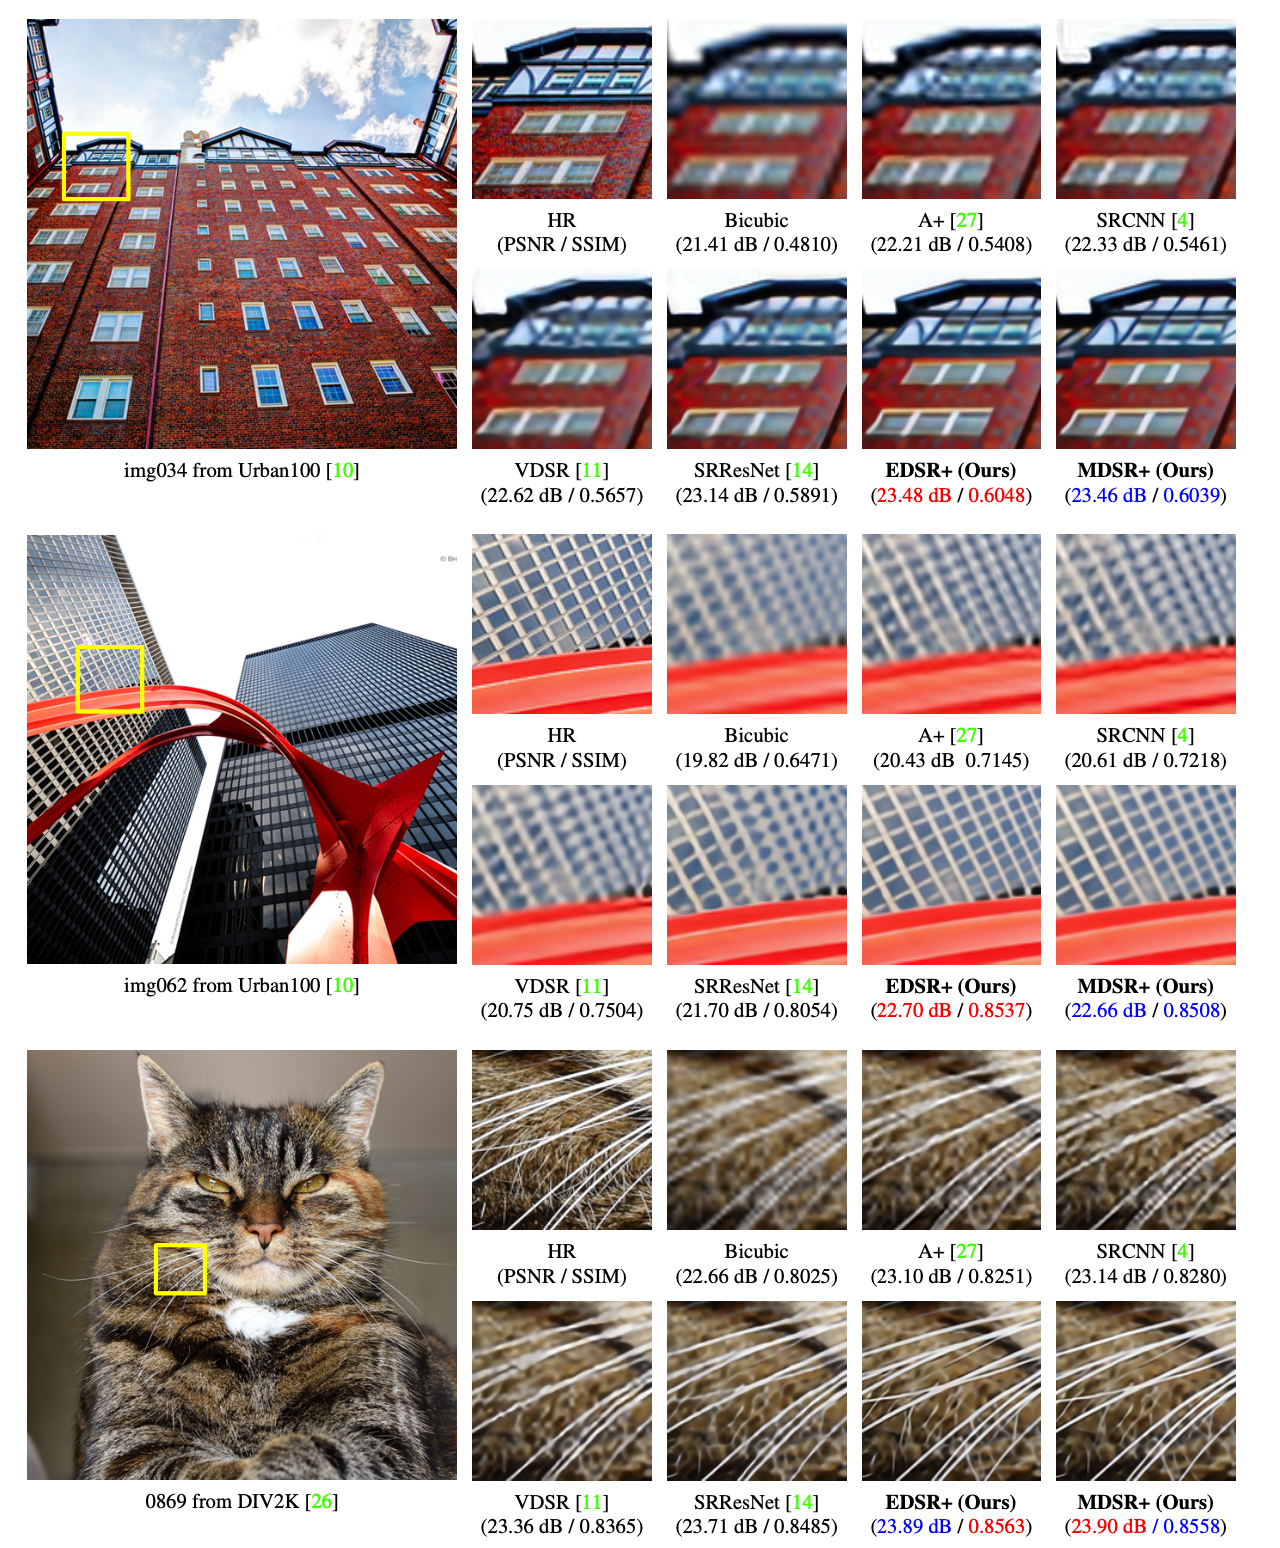
\includegraphics[width=\textwidth]{compare_SR}
  \caption[Comparison of different Super-resolution models.]{Comparison of different Super-resolution models. HR is raw high resolution image taken. Adapted from \cite{EDSR}}
  \label{fig:compare_SR}
\end{figure}
